\documentclass[11pt]{article}
\usepackage[margin=1in]{geometry}
\usepackage{amsmath,amssymb,booktabs,tabularx,array,graphicx,hyperref}
\newcolumntype{Y}{>{\raggedright\arraybackslash}X}
\title{Semantic Epistemic Risk versus Confidence-Based Active Retrieval During Generation}
\author{Working Draft}\date{August 2026}
\begin{document}\maketitle

\begin{abstract}
Active retrieval during generation is established prior art: FLARE retrieves
when forecast tokens have low model confidence \cite{flare}. We ask whether
uncertainty is equivalent to epistemic risk. Using one versioned controlled
source, we freeze 80 untouched Qwen-measured test examples with exactly 20 in
each confidence--retrieval-requirement quadrant, then evaluate Qwen3-0.6B,
SmolLM2-1.7B, and Gemma3-1B. A transparent semantic trigger has 100\% retrieval
recall and 2.5\% false activation on all three families. Confidence-only recall
is 50\%, 0\%, and 97.5\%, respectively, exposing strong checkpoint calibration
dependence. A deterministic runtime epistemic gate reduces Unsupported
Commitment Rate (UCR) from 100\% unassisted to 0\% for every model while
retrieving less than upfront RAG; accuracy is 97.5\%, 96.25\%, and 77.5\%, so
enforcement can trade utility for support. A secondary placement experiment is
negative: three rank-8 LoRA adapters achieve near-zero synthetic development
loss but collapse to zero held-out retrieval recall. Gemma in-context learning
reaches full recall but only 36.25\% valid-interface success. Under this freeze,
stable retrieval policy belongs in the transparent runtime, not the tested
context or weights. The multi-source Paper 2.5 gate passes, but learned source
routing is not implied.
\end{abstract}

\section{Question and Claim Boundary}
The primary question is: \emph{is epistemic risk distinct from model
uncertainty?} Retrieval-required means that a reliable answer depends on an
external or source-specific record rather than model weights or already supplied
active context. This operational label is distinct from model confidence.

The secondary question is placement: \emph{where should stable one-source
interface knowledge live: context, weights, or runtime?} Phase B begins only
after the Phase A source, benchmark, confidence probes, threshold objective, and
evaluation are frozen. The paper does not claim active retrieval itself as novel
and does not study multi-source routing.

\section{Mechanism}
\[
Q\rightarrow y_{1:t}\rightarrow \widehat{y}_{t+1:t+k}
\rightarrow \{T_{\mathrm{conf}},T_{\mathrm{sem}}\}
\rightarrow \text{retrieve}\rightarrow \text{evidence/status}
\rightarrow \text{accept or abstain}.
\]
The FLARE-like controller greedily forecasts one short answer span, records the
probability of every forecast token, triggers on the minimum probability, and
regenerates with evidence. Canonical FLARE forecasts longer text, may mask
uncertain spans, and iterates during long-form generation \cite{flare}; our
single-opportunity controlled diagnostic is not a canonical reproduction.

The semantic controller uses answer-independent lexical, entity, temporal,
freshness, source-dependence, and active-context rules. It has an explicit
exception for ``electric current'' and treats compute requests as belonging to a
different coprocessor. Rules never contain source answer values.

\section{Controlled Source and Evidence Policy}
The frozen source is
\texttt{atlas-controlled-registry@2026.08.2-frozen-candidates}. Records have
stable IDs, validity intervals, source version, and provenance. They cover
stable, superseded familiar, unfamiliar private, unavailable, and conflicting
facts. Requests contain entity, attribute, as-of date, forecast, source version,
and resource bounds. Outcomes include \textsc{supported},
\textsc{contradicted}, \textsc{unverified}, \textsc{stale},
\textsc{ambiguous}, and \textsc{conflict}.

The runtime gate enforces support relative to this configured source; it does
not establish truth. A unique supported value may be accepted. Missing,
ambiguous, or conflicting evidence forces abstention rather than an unsupported
factual commitment.

\section{Frozen Measured-Quadrant Benchmark}
We generate 256 candidates: 32 development and 224 candidate-test examples.
Confidence is measured on pinned Qwen3-0.6B before test selection. The
development threshold maximizes retrieval-requirement F1 minus 0.25 times
retrieval rate and equals 0.84993. The candidate pool contains 25, 87, 22, and 90
examples in the four observed Qwen quadrants; the freezer selects exactly 20
from each. IDs are fixed before any condition evaluation.

Retrieval-required subclasses are fresh/current, source-version-specific,
private, changed familiar, unavailable, conflicting, exact attribution, and
structured one-source values. Retrieval-not-required subclasses are stable
facts, supplied context, freshness distractors, quotations, hypotheticals,
non-factual prose, and compute needs. The final benchmark contains 32 development
and 80 untouched test examples.

Each model independently fits its threshold on the common development set:
0.84993 for Qwen, 0.14693 for SmolLM2, and 0.99971 for Gemma. Qwen and Gemma
observe all four test quadrants. SmolLM2 places no test example below its fitted
threshold, so its test set lacks low-confidence quadrants. This is a calibration
result and limits cross-model quadrant claims.

\section{Conditions and Metrics}
Phase A has 13 conditions: LLM only, anti-hallucination prompting, upfront RAG,
explicit retrieval, FLARE-like confidence, semantic, confidence OR semantic,
confidence AND semantic, retrospective verification, evidence advisory,
evidence plus abstention instruction, runtime epistemic gate, and oracle.

UCR is the fraction of retrieval-required opportunities that emit an unsupported
factual commitment. Authorized Commitment Coverage is the fraction of
non-abstention retrieval-required opportunities answered with the authorized
value. We also report exact accuracy, retrieval precision/recall and rate,
confident-hallucination catch rate, quadrant retrieval, runtime enforcement,
generated tokens, calls, and wall time. Accuracy intervals and complete
threshold sweeps are machine-readable.

\section{Phase A Results}
All runs use greedy decoding, seed 17, pinned revisions, PyTorch 2.13.0+XPU, and
Intel integrated graphics. Each family produces 1,456 prediction rows and 1,456
traces. Table~\ref{tab:phase-a} reports the primary conditions.

\begin{table}[t]
\centering\scriptsize
\caption{Untouched 80-example Phase A test. Acc.=exact accuracy,
Ret.=retrieval rate, Cov.=Authorized Commitment Coverage.}
\label{tab:phase-a}
\begin{tabular}{@{}llcccc@{}}
\toprule
Model & Condition & Acc. & Ret. & UCR & Cov.\\
\midrule
Qwen & LLM only & .238 & .000 & 1.000 & .000\\
     & FLARE-like & .625 & .500 & .675 & .325\\
     & Semantic & .613 & .513 & .250 & .750\\
     & Conf. OR semantic & .838 & .763 & .250 & .750\\
     & Runtime gate & .975 & .763 & .000 & 1.000\\
     & Upfront RAG & .850 & 1.000 & .250 & .750\\
\midrule
SmolLM2 & LLM only & .463 & .000 & 1.000 & .000\\
        & FLARE-like & .463 & .000 & 1.000 & .000\\
        & Semantic & .575 & .513 & .775 & .225\\
        & Conf. OR semantic & .575 & .513 & .775 & .225\\
        & Runtime gate & .963 & .513 & .000 & 1.000\\
        & Upfront RAG & .400 & 1.000 & .775 & .225\\
\midrule
Gemma & LLM only & .463 & .000 & 1.000 & .000\\
      & FLARE-like & .813 & .900 & .325 & .675\\
      & Semantic & .800 & .513 & .300 & .700\\
      & Conf. OR semantic & .825 & .913 & .300 & .700\\
      & Runtime gate & .775 & .913 & .000 & 1.000\\
      & Upfront RAG & .825 & 1.000 & .300 & .700\\
\bottomrule
\end{tabular}
\end{table}

Confidence and semantic risk are not equivalent. Qwen confidence retrieves both
low-confidence quadrants, giving 50\% recall and 50\% false intervention; the
semantic rule retrieves all 40 required cases and one of 40 controls. SmolLM2's
fitted confidence retrieves nothing. Gemma confidence has 97.5\% recall but
82.5\% false activation. The same semantic policy has 100\% recall and 2.5\%
false activation on all three because it is independent of checkpoint logits.

The runtime gate eliminates unsupported commitments in every family. It also
shows why reliability and answer accuracy must be separated: Qwen and SmolLM2
improve sharply, whereas Gemma drops five accuracy points below upfront RAG.
Enforcement prevents unsupported acceptance but cannot guarantee that the base
answer or abstention policy maximizes exact-match utility.

\begin{figure}[t]
\centering
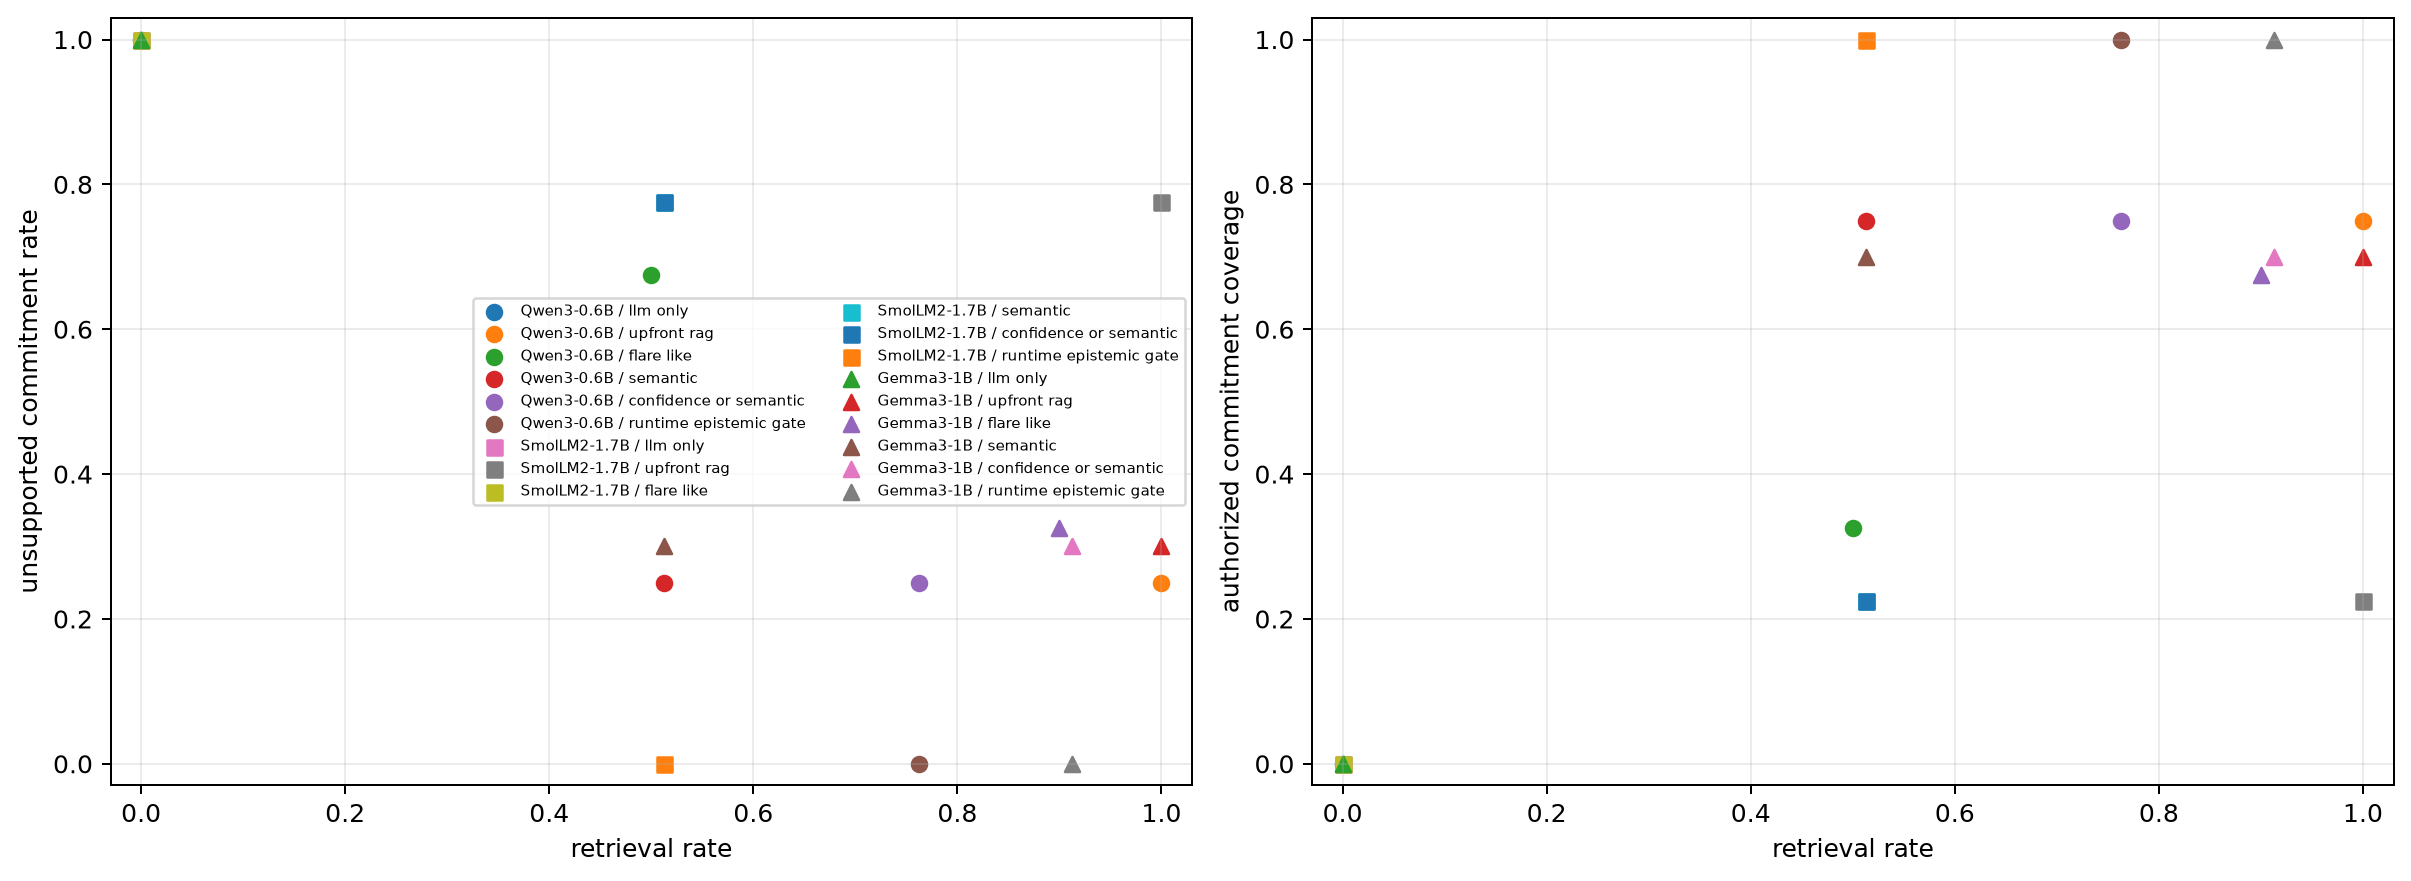
\includegraphics[width=0.96\linewidth]{paper1_5_ucr_coverage.png}
\caption{Retrieval cost against UCR and Authorized Commitment Coverage across
three checkpoints. The runtime gate reaches zero UCR but has model-dependent
accuracy consequences.}
\label{fig:phase-a}
\end{figure}

\section{Phase B: Context, Weights, or Runtime}
The adapter dataset contains 160 balanced training rows and 40 development rows
with disjoint entity namespaces and values. It excludes every held-out benchmark
entity and answer. Targets contain either a four-field \texttt{retrieve} block or
\texttt{NO\_RETRIEVAL}; no target contains an answer value. The overlap audit has
zero train/development, held-out entity, or held-out value collisions.

Rank-8 adapters train for two epochs on Qwen, SmolLM2, and Gemma. Final
development losses are 0.00028, 0.0004, and 0.0001. This apparent fit does not
transfer. Table~\ref{tab:placement} compares held-out policy selection. Interface
success additionally requires the correct entity, attribute, date, and source.
Prompt-token values are measured condition totals; the runtime semantic rows use
the Phase A answer template and are not a matched estimate of policy-only prompt
overhead.

\begin{table}[t]
\centering\scriptsize
\caption{Held-out 80-example placement evaluation. Sel.=selection accuracy,
Int.=valid interface success, Rec.=retrieval recall, FA=false activation.}
\label{tab:placement}
\begin{tabular}{@{}llcccccc@{}}
\toprule
Model & Placement & Sel. & Int. & Rec. & FA & Prompt tok. & Gen. tok.\\
\midrule
Qwen & Context & .500 & .500 & .000 & .000 & 136.6 & 6.2\\
     & Weights & .500 & .500 & .000 & .000 & 67.6 & 6.0\\
     & Runtime semantic & .988 & .988 & 1.000 & .025 & 101.4 & 10.2\\
\midrule
SmolLM2 & Context & .050 & .013 & .075 & .975 & 172.2 & 31.4\\
        & Weights & .500 & .500 & .000 & .000 & 91.2 & 7.0\\
        & Runtime semantic & .988 & .988 & 1.000 & .025 & 137.0 & 8.2\\
\midrule
Gemma & Context & .863 & .363 & 1.000 & .275 & 139.0 & 24.4\\
      & Weights & .500 & .500 & .000 & .000 & 66.0 & 5.8\\
      & Runtime semantic & .988 & .988 & 1.000 & .025 & 101.1 & 8.3\\
\bottomrule
\end{tabular}
\end{table}

All adapters collapse to \texttt{NO\_RETRIEVAL}: zero recall, no false
activation, and 50\% balanced selection accuracy. Qwen context behaves the same.
SmolLM2 context mostly over-triggers and often emits invalid blocks. Gemma
context detects all needs but only 36.25\% of all examples pass the complete
interface criterion. Adding confidence to adapter outputs does not recover Qwen
or SmolLM2 and inherits Gemma confidence's 82.5\% false activation.

\begin{figure}[t]
\centering
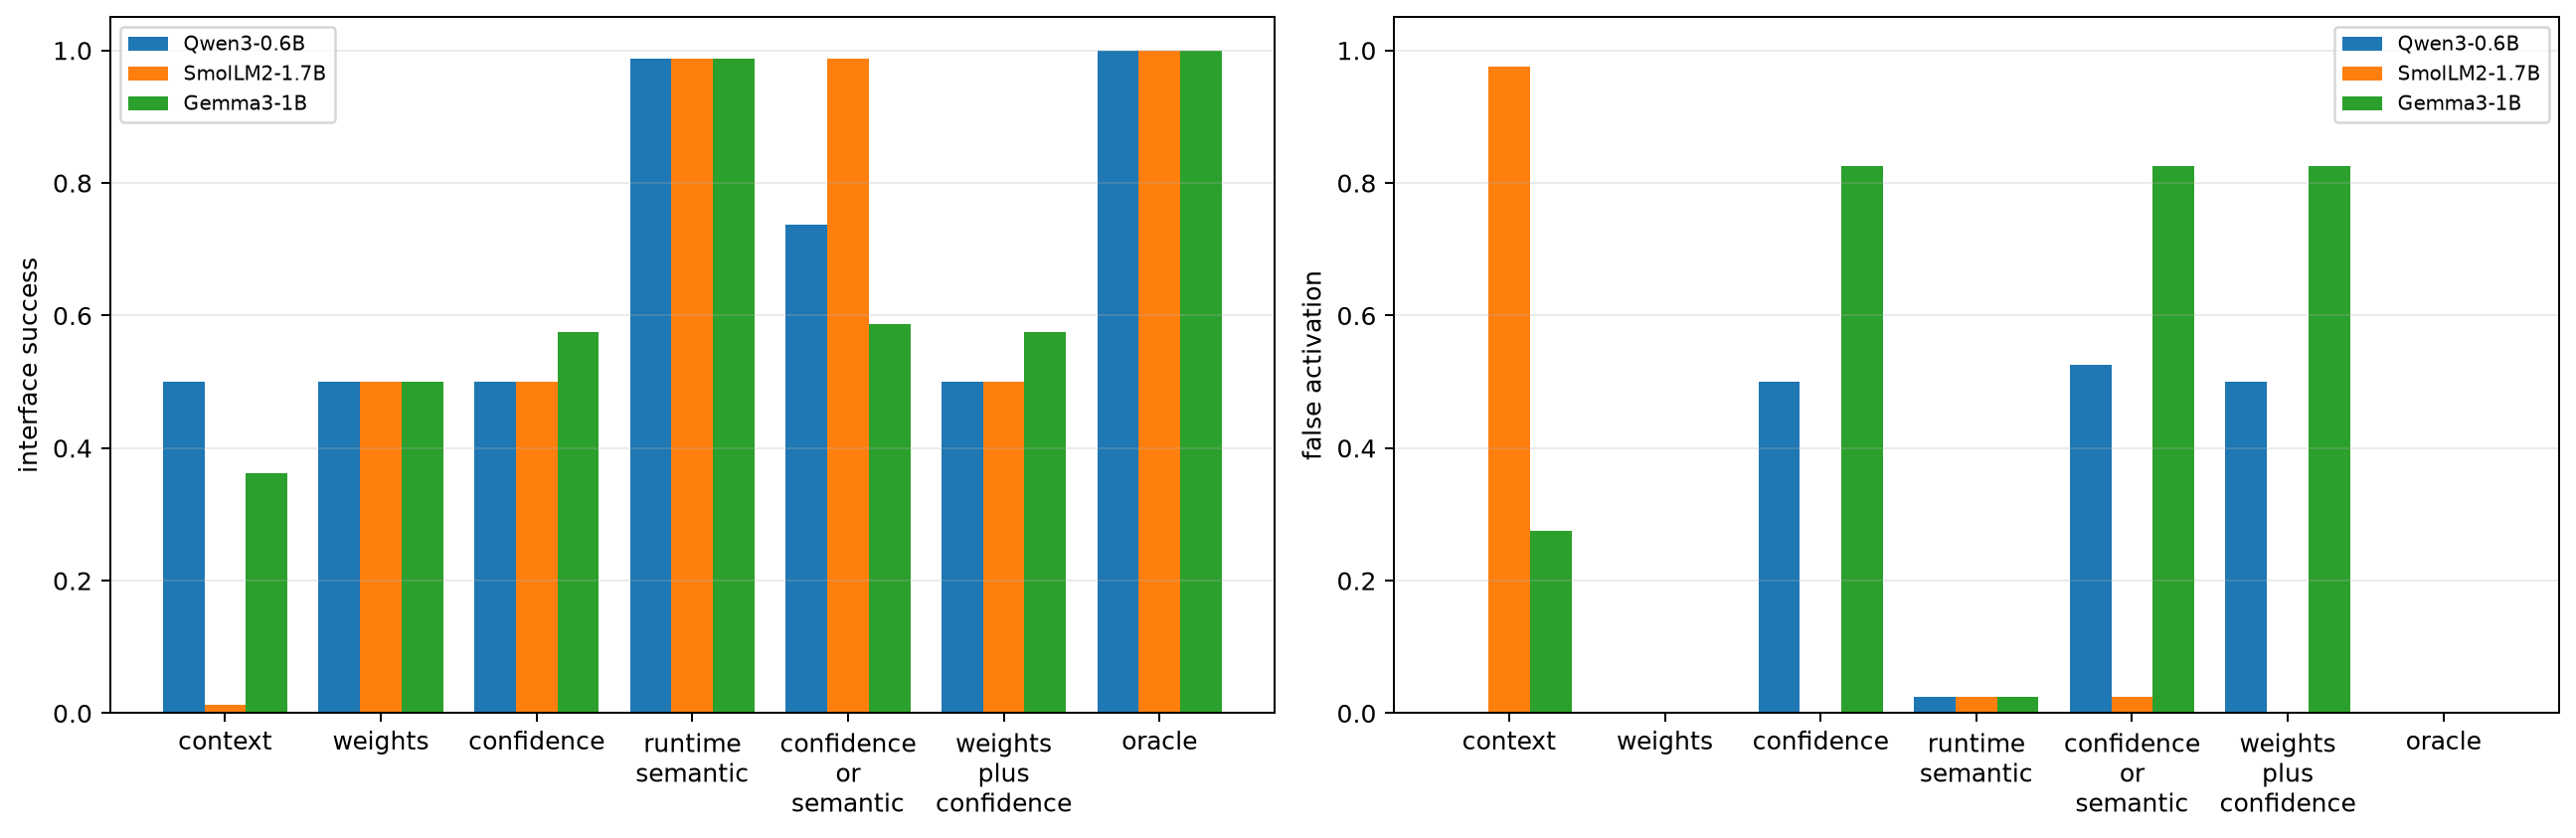
\includegraphics[width=0.98\linewidth]{paper1_5_policy_placement.png}
\caption{Interface success and false activation for context, weights,
confidence, transparent runtime semantics, combinations, and oracle.}
\label{fig:placement}
\end{figure}

Near-zero development loss alongside zero held-out recall is direct evidence of
protocol overfitting to narrow synthetic phrasing. It falsifies the proposed
weight-placement benefit under this training design. More diverse training may
change that result, but adapting after inspecting these held-out failures would
require a new freeze.

\section{Paper 2.5 Gate}
The pre-registered gate asks whether at least two families reduce UCR with the
runtime gate while retrieving less often than upfront RAG. Qwen, SmolLM2, and
Gemma all pass; Paper 2.5 is therefore \textsc{go}. This authorizes testing
source heterogeneity. It does not authorize learned source routing, because
Phase B provides no evidence that the retrieval policy should move into weights.

\section{Falsification and Limitations}
The primary result would be weakened if a better-calibrated FLARE implementation
matches semantic routing at equal cost, if natural-language semantic rules lose
precision, or if the confident-risk quadrants disappear on new data. The present
result instead finds checkpoint-dependent confidence behavior and stable rule
recall, but only on one controlled source and synthetic short answers.

The benchmark is selected using Qwen confidence, so its exact 20-per-quadrant
balance does not transfer to other checkpoints. SmolLM2 lacks low-confidence test
examples. There is one seed per model, no long-form repeated retrieval, and no
ranking noise. The semantic cue distribution is controlled. The runtime gate is
deterministic and answer-aware relative to source evidence, not a production
truth system. Full-prefix generation latency is not production latency.

Phase B uses narrow train templates despite strict entity/value leakage controls;
its failure may be covariate shift rather than a general limitation of LoRA.
Conversely, development loss is clearly not evidence of interface
generalization. The ICL baseline uses textual examples rather than native tool
schemas. No condition trains or tests multi-source selection.

\section{Reproduction}
Paper-specific code is under \texttt{src/ccpu/paper1\_5}. From the repository
root, activate the validated XPU environment and run:
\begin{verbatim}
$py = 'C:\Users\j.simao\.venvs\modal-llm-xpu\Scripts\python.exe'
$env:PYTHONPATH = (Resolve-Path src).Path
& $py -m ccpu paper1.5 freeze-next \
  --config configs/paper1_5/next_iter_freeze_qwen_xpu.json \
  --output-dir artifacts/paper1_5/next_iter/freeze_qwen_v2
& $py -m ccpu paper1.5 run-hf \
  --config configs/paper1_5/next_iter_qwen_xpu.json \
  --output-dir artifacts/paper1_5/next_iter/qwen_v2
python -m ccpu paper1.5 analyze-next \
  --config configs/paper1_5/next_iter_analysis.json \
  --output-dir artifacts/paper1_5/next_iter/analysis_v1
& $py -m ccpu paper1.5 train-policy-lora <arguments in README>
python -m ccpu paper1.5 analyze-policy \
  --config configs/paper1_5/policy_placement.json \
  --output-dir artifacts/paper1_5/next_iter/policy_analysis_v1
\end{verbatim}
Manifests hash configurations, benchmark/source snapshots, predictions, traces,
summaries, and adapter files and record checkpoint revisions, device, package,
repository, and environment provenance.

\section{Conclusion}
Semantic epistemic risk adds information beyond checkpoint uncertainty in this
controlled one-source regime. A runtime gate eliminates unsupported commitments
for three small model families at lower retrieval cost than upfront RAG, although
Gemma exposes an accuracy cost. The placement extension is negative: context is
inconsistent and the tested adapters overfit. For the current freeze, exact
source mechanics and enforcement clearly belong in runtime, and stable semantic
selection should remain transparent there until independently frozen training
demonstrates weight-policy generalization.

\begin{thebibliography}{9}
\bibitem{flare}
Z.~Jiang et al. Active retrieval augmented generation. \emph{EMNLP}, 2023.
\url{https://arxiv.org/abs/2305.06983}.
\end{thebibliography}
\end{document}
